\hypertarget{nuxe1stroje-pro-pruxe1ci-s-derivacuxed-v-ux10deskuxe9m-prostux159eduxed}{%
\chapter{Nástroje pro práci s~derivací v~českém
prostředí}\label{nuxe1stroje-pro-pruxe1ci-s-derivacuxed-v-ux10deskuxe9m-prostux159eduxed}}

Na základě onomaziologické teorie Miloše Dokulila (a~jeho následovníků)
vzniklo nemalé množství počítačových programů, prostřednictvím kterých
lze dosahovat různých výzkumných, edukačních či komerčních výsledků,
proto si v~první část této kapitoly popíšeme nejvýznamnější softwarové
nástroje, které se využívají pro práci s~derivací v~českém prostředí.
V~druhé části si pak hlouběji představíme derivační síť Derinet, na níž je
postaveno řešení praktické části této bakalářské práce.

\hypertarget{pux159ehled-nuxe1strojux16f}{%
\section{Přehled nástrojů}\label{pux159ehled-nuxe1strojux16f}}

\hypertarget{morfio}{%
\subsection{Morfio}\label{morfio}}

Webová aplikace Morfio je jedním z~projektů Českého národního korpusu,
která „slouží k~odhadování rozsahu a~produktivity slovotvorných modelů
v~češtině na základě korpusových dat``. Jde tedy o~systém, který se snaží
ve zvoleném korpusu najít takové n-tice slov, které se shodují určitým
slovotvorným základem a~liší se specifickým slovotvorným formantem (těch
může být i~více, navíc je zde reflektována problematika hláskových
alternací.) Nástroj je tedy vhodný spíše jako výzkumná pomůcka než-li
jako prostředek ke tvorbě relevantních lingvistických výstupů, protože
při manipulaci s~korpusovými daty, jež nejsou nijak sémanticky
označkována, může docházet k~chybám například z~důvodu homonymie.
\parencite{cvrcek13}

\hypertarget{morfologickuxe9-analyzuxe1tory-ajka}{%
\subsection{Morfologické analyzátory
Ajka}\label{morfologickuxe9-analyzuxe1tory-ajka}}

Dalším nástrojem je morfologický analyzátor Ajka (vyvinutý na Masarykově
univerzitě), jehož hlavní složkou je analýza flektivní morfologie -- to
znamená, že obsahuje rozsáhlý systém vzorů spolu se sadami určitých
koncovek a~morfologických značek. Ve webovém rozhraní je možnost vstupní
text buď segmentovat na jednotlivé morfologické segmenty, analyzovat
z~pohledu určitého paradigmatu nebo vyhledat existující akcentovaný výraz
(například pro vstup \emph{blázen} je výstupem výraz \emph{blažen}).
Nástroj nicméně akcentuje i~složku derivační, a~to ve formě
hierarchického systému morfologických paradigmat, který slouží pro
zachycení všech úrovní derivační morfologie.~\parencite{ajka}

V~průběhu času vznikl z~potřeby efektivnějšího zpracování textu
z~morfologického analyzátoru Ajka nástroj Majka, který používá stejná
jazyková data, ale kompletně proměnil jejich formát a~stejně tak
algoritmus, který nad nimi operuje -- tak bylo docíleno větší rychlosti
zpracování.~\parencite{majka}

\hypertarget{deriv}{%
\subsection{Deriv}\label{deriv}}

Třetím relevantním softwarovým řešením zabývající se slovní derivací je
projekt Masarykovy univerzity Deriv, jenž je víceúčelovým nástrojem pro
automatické zpracování přirozeného jazyka s~primárním cílem testovat
možnosti automatické slovotvorné analýzy. Jeho webového rozhraní se
skládá ze dvou základních funkcí -- vyhledávání podle formálního zadání
a~kategorizace vyhledaných dat. Samotný Deriv je založený na
automatickém morfologickém analyzátoru Ajka (později Majka), v~rámci
kterého využívá jeho morfologický slovník kmenů a~vyhledává v~něm
prostřednictvím morfologických značek a~regulárních
výrazu\footnote{Nástroj využívá regulární výrazy programovacího jazyka Perl verze 5.10 a~novější.}.
Velkou výhodou aplikace je fakt, že jsou výsledky hledání propojeny
s~českými výkladovými slovníky (SSČ, SSJČ, PSJČ) a~s~některými českými
korpusy (konkrétně CzTenTen, SYN2000).~\parencite{deriv}

\hypertarget{derivancze}{%
\subsection{Derivancze}\label{derivancze}}

Předposledním rozebíraným nástrojem je derivační analyzátor Derivancze,
který analyzuje slovotvorné vztahy mezi slovy. Využívá veřejně přístupná
data derivační sítě Derinet, ale na rozdíl od ní pracuje pouze se
sémantickými vztahy, to znamená, že pokud se liší formální a~významový
aspekt derivačního vztahu, tak je vyžadováno explicitní označkovaní,
díky kterému pak dochází ke konzistenci napříč daty. Nástroj využívá
sedmnácti značek označující typ sémantického vztahu -- může jít
například o~značku \emph{k1ag}, která označuje vztah odvození verba
směrem k~činitelskému jménu. Nicméně tento přístup vytváří určité
problémy, nastroj je problematické použit v~rámci větších
sofistikovanějších aplikací (například automatické generování textu),
protože by bylo zapotřebí dodat více informací o~typech jednotlivých
slovotvorných vztahů.~\parencite{derivancze}

\hypertarget{derivaux10dnuxed-suxedux165-derinet}{%
\section{Derivační síť
Derinet}\label{derivaux10dnuxed-suxedux165-derinet}}

Text.

\begin{center}
    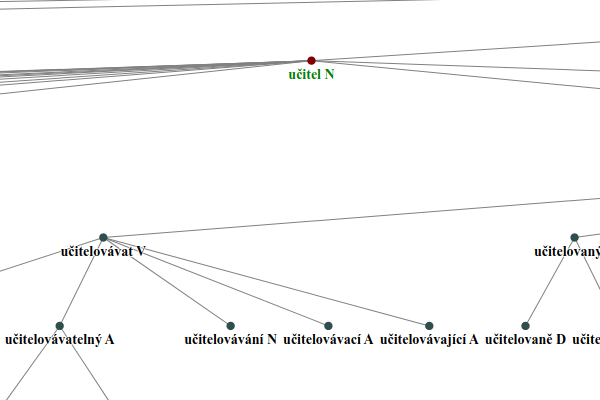
\includegraphics{derinet}
\end{center}

Text.~\parencite{derinet-cz}
